\documentclass[12pt,letterpaper]{article}

% Essential packages for patent formatting
\usepackage[top=1in, bottom=1in, left=1in, right=1in]{geometry} % Proper margins
\usepackage{setspace} % For 1.5 or double line spacing
\usepackage{times} % Times Roman font (or use \usepackage{helvet} for Arial)
\usepackage{enumitem} % For customizing lists/enumerations in claims
\usepackage{fancyhdr} % For headers
\usepackage{titlesec} % For section formatting
\usepackage{graphicx} % For including drawings
\usepackage{amsmath} % For mathematical equations
\usepackage{amssymb} % For mathematical symbols
\usepackage{physics} % For quantum mechanics notation
\usepackage{braket} % For quantum state notation
\usepackage{lipsum} % For sample text (remove in actual document)
\usepackage{tikz}
\usetikzlibrary{arrows.meta,positioning,shapes.geometric,calc,decorations.pathmorphing,intersections,patterns}
\usepackage{pgfplots}
\pgfplotsset{compat=1.17}

% Set the line spacing to 1.5 (or 2.0 for double spacing)
\onehalfspacing
% \doublespacing  % Uncomment for double spacing

% Configure headers and footers
\pagestyle{fancy}
\fancyhf{} % Clear all headers and footers
\renewcommand{\headrulewidth}{0pt} % Remove header rule
\fancyfoot[C]{\thepage} % Page number at bottom center

% Configure section formatting
\titleformat{\section}
  {\normalfont\bfseries\uppercase}
  {}
  {0em}
  {}
\titlespacing{\section}{0pt}{12pt}{6pt}

% Configure subsection formatting
\titleformat{\subsection}
  {\normalfont\bfseries}
  {}
  {0em}
  {}
\titlespacing{\subsection}{0pt}{12pt}{6pt}

% Custom paragraph format with additional spacing
\setlength{\parindent}{0pt}
\setlength{\parskip}{6pt}

% Custom enumeration for claims
\newlist{patentclaims}{enumerate}{2}
\setlist[patentclaims,1]{label=\arabic*., align=left, leftmargin=2em, itemsep=1em}
\setlist[patentclaims,2]{label=\arabic*., align=left, leftmargin=2em, itemsep=0.5em}

\begin{document}

% ===== TITLE PAGE =====
\begin{center}
\Large\bfseries
SYSTEM AND METHOD FOR MULTI-PHOTON DETECTION USING QUANTUM DOT ARRAYS WITH WAVEFUNCTION-GUIDED SPECTRAL SELECTIVITY
\end{center}

\vspace{0.5in}

\vspace{1in}

\section*{CROSS-REFERENCE TO RELATED APPLICATIONS}

This application is related to co-pending U.S. Patent Application titled "SYSTEM AND METHOD FOR TEMPORAL PROCESSING USING MULTI-SHELL ARCHITECTURE WITH CONFIGURABLE COUPLING," filed concurrently herewith, the entire contents of which are hereby incorporated by reference. The multi-photon detection capabilities described herein can be integrated with the temporal shell architecture described in the related application to enable enhanced temporal-spectral processing capabilities.

\section*{FIELD OF THE INVENTION}

The present invention relates to quantum photonics, and more particularly to multi-photon detection systems with spectral discrimination capabilities. Specifically, the invention pertains to systems and methods for detecting multiple simultaneous photons across different wavelengths using engineered quantum dot arrays with wavefunction-guided spectral selectivity, with applications in quantum information processing, quantum communication, and advanced optical sensing.

\section*{BACKGROUND}

In the field of quantum photonics, accurate detection and measurement of multiple photons are critical for applications ranging from quantum information processing to advanced spectroscopy. Conventional photon detection systems typically employ single-photon avalanche diodes (SPADs), superconducting nanowire single-photon detectors (SNSPDs), or photomultiplier tubes (PMTs) in conjunction with spectral filtering elements to separate photons of different wavelengths.

These conventional approaches suffer from several limitations. First, they generally require photon splitting and routing to multiple detector elements when measuring multiple photons, resulting in reduced detection efficiency and increased system complexity. This splitting introduces path-dependent losses and temporal synchronization challenges that degrade system performance for quantum correlation measurements. Second, spectral discrimination in conventional systems relies on passive optical elements such as diffraction gratings or dichroic filters, which impose fixed spectral resolution limits and exhibit crosstalk between adjacent spectral channels.

Quantum dot (QD) based photodetectors represent an alternative approach, utilizing the discrete energy levels of semiconductor quantum dots to detect photons. However, existing QD photodetectors typically operate with each quantum dot functioning as an independent absorption and detection center, failing to leverage quantum mechanical interactions between multiple quantum dots. Furthermore, current QD detector systems primarily operate in a classical regime where photon absorption triggers carrier generation and electrical current flow, without preserving or utilizing quantum information contained in the incoming photon's quantum state.

Recent advances in engineered quantum systems have demonstrated the possibility of coherent interactions between quantum dots through wavefunction engineering. For instance, coupled quantum dot systems have been developed for quantum computing applications where electron wavefunctions overlap to enable quantum gate operations. However, these principles have not been effectively translated to the domain of photon detection with spectral discrimination capabilities.

Therefore, there remains a need for a photon detection system that can simultaneously detect multiple photons while providing precise spectral discrimination, without requiring photon splitting or complex optical filtering arrangements. Such a system would ideally preserve quantum correlations between detected photons and enable reconfigurable spectral selectivity through wavefunction engineering rather than fixed optical elements.

\section*{SUMMARY}

The present invention addresses the aforementioned limitations by providing a system and method for simultaneous detection of multiple photons across different wavelengths using an engineered quantum dot array with wavefunction-guided spectral selectivity. In one aspect, the invention comprises a quantum dot array with engineered energy levels and geometric configuration optimized for multi-photon detection, a mechanism for projecting incoming photon states onto the quantum dot array basis, and a processing system for reconstructing the original photon state through temporal correlation analysis.

An advantage of the present invention is the ability to simultaneously detect multiple photons while preserving their quantum correlations, enabling applications in quantum information processing that require intact quantum states. Additionally, the invention allows for reconfigurable spectral selectivity through electronic control of the quantum dot parameters, rather than requiring fixed optical filtering elements.

In various embodiments, the invention may include integrated quantum state tomography capabilities, adaptive wavefunction optimization based on detected photon statistics, and interfaces with quantum memory systems to further enhance quantum information processing capabilities.

\section*{BRIEF DESCRIPTION OF THE DRAWINGS}

% INSTRUCTIONS: List each figure number with a brief description of what it shows. Every drawing must be described, and every element referenced in the Detailed Description must appear in at least one drawing. For AI prompting: "Create a list of figure descriptions where each entry briefly describes what that figure shows. Use the format 'FIG. X is a [type of view/diagram] of [what it shows].' Include all perspectives needed to understand the invention's physical structure and operation."

FIG. 1 is a block diagram illustrating the overall system architecture of the multi-photon detection system according to an embodiment of the present invention.

FIG. 2 is a schematic diagram depicting the physical arrangement of a quantum dot array with engineered energy levels according to an embodiment of the present invention.

FIG. 3 is a cross-sectional view of a single quantum dot structure within the quantum dot array.

FIG. 4 is an energy-level diagram illustrating the engineered quantum dot energy states and their relationship to photon detection across multiple wavelengths.

FIG. 5 is a schematic representation of wavefunction overlap between adjacent quantum dots in the array, showing the basis for wavefunction-guided spectral selectivity.

FIG. 6 is a flowchart depicting the method for multi-photon detection using the quantum dot array system.

FIG. 7 is a graph showing spectral response characteristics of the quantum dot array compared to conventional photon detection systems.

FIG. 8 is a schematic diagram of the readout circuit architecture for the quantum dot array.

FIG. 9 is a block diagram of the signal processing subsystem for temporal correlation analysis and photon state reconstruction.

FIG. 10 is a diagram illustrating an alternative embodiment with integrated quantum memory elements.

\section*{DETAILED DESCRIPTION}

% INSTRUCTIONS: Provide a complete and enabling disclosure of your invention. Describe each embodiment in detail using reference numbers that match your drawings. Explain structure, function, and operations. This is the longest section (typically 5-20 pages). For AI prompting: "Explain the invention in extensive detail, describing at least one complete embodiment with reference to drawing element numbers (e.g., widget 101). Describe physical structure, functional relationships, materials, dimensions where relevant, manufacturing methods, and operational procedures. The description must enable a skilled person to make and use the invention without undue experimentation."

The following detailed description refers to the accompanying drawings which form a part of this disclosure. In the drawings, similar symbols typically identify similar components, unless context dictates otherwise. The illustrative embodiments described herein are not meant to be limiting. Other embodiments may be utilized, and other changes may be made, without departing from the spirit or scope of the subject matter presented here.

Referring first to FIG. 1, a multi-photon detection system 100 includes a quantum dot array 101 connected to a readout circuit 102 and a signal processing subsystem 103. The quantum dot array 101 forms the core detection element of the system and is formed of a semiconductor substrate hosting multiple engineered quantum dots arranged in a specific geometric configuration optimized for multi-photon detection.

The readout circuit 102 is electronically coupled to the quantum dot array 101 via interconnects 104 and functions to convert quantum state information from the quantum dot array into electrical signals that can be processed by the signal processing subsystem 103. The signal processing subsystem 103 receives electrical signals from the readout circuit 102 through data transmission lines 105 and performs temporal correlation analysis and quantum state reconstruction.

The system 100 further includes an optical input interface 106 positioned to direct incoming photons onto the quantum dot array 101, and a control system 107 electronically connected to the quantum dot array 101, readout circuit 102, and signal processing subsystem 103 via control lines 108. The control system 107 functions to adjust operational parameters of the entire system, including quantum dot energy levels, readout timing, and signal processing algorithms.

As shown in FIG. 2, the quantum dot array 101 includes multiple quantum dots 201, 202, 203, 204, and 205 arranged in a specific geometric pattern on a semiconductor substrate 206. The quantum dots are positioned at precisely calculated distances from each other to optimize wavefunction overlap between adjacent dots. In the exemplary embodiment shown, the quantum dots are arranged in a pentagonal configuration, though other geometric arrangements may be utilized depending on the specific application requirements.

Each quantum dot 201-205 has individually addressable gate electrodes 207 connected to control lines 208 that extend to the control system 107. These gate electrodes 207 allow for precise tuning of the energy levels of individual quantum dots through application of controlled electric fields, enabling reconfigurable spectral selectivity of the detection system.

Referring now to FIG. 3, which shows a cross-sectional view of a single quantum dot structure 201, the internal structure can be observed. The quantum dot comprises a core semiconductor material 301 surrounded by a higher bandgap barrier material 302. The core semiconductor material 301 is selected from the group consisting of InAs, InGaAs, GaAs, CdSe, PbS, or other suitable semiconductor materials that provide the desired quantum confinement properties. The barrier material 302 is selected to have a wider bandgap than the core material, and may consist of GaAs, AlGaAs, InP, or other suitable materials that provide sufficient energy barriers for carrier confinement.

The quantum dot structure 201 further includes a gate electrode 207 positioned above the dot and separated from it by a thin dielectric layer 303. The gate electrode 207 is formed of a conductive material such as gold, aluminum, or doped polysilicon. The dielectric layer 303 consists of materials such as SiO$_2$, HfO$_2$, or Al$_2$O$_3$ with a thickness ranging from 5 to 20 nanometers. Contact leads 304 connect the quantum dot to the readout circuit 102 and allow for measurement of the quantum dot's state.

The quantum dot 201 has physical dimensions carefully engineered to produce the desired energy level structure. In typical embodiments, the quantum dot has a diameter ranging from 3 to 20 nanometers and a height ranging from 2 to 10 nanometers, though these dimensions may be varied depending on the target spectral response characteristics of the system.

FIG. 4 illustrates the energy-level diagram of the engineered quantum dot energy states and their relationship to photon detection. Each quantum dot (represented as QD1 401, QD2 402, and QD3 403) is engineered to have specific discrete energy levels. The ground state energy level is represented as $E_0$ (411, 421, 431), while the excited states are labeled as $E_1$ (412, 422, 432), $E_2$ (413, 423, 433), and so forth. 

The energy difference between the ground state and various excited states corresponds to the energies of photons that can be detected. For example, a photon with energy $\hbar\omega_1$ 441 can excite an electron from the ground state $E_0$ 411 to the excited state $E_1$ 412 in quantum dot QD1 401. Similarly, photons with energies $\hbar\omega_2$ 442 and $\hbar\omega_3$ 443 can excite transitions in quantum dots QD2 402 and QD3 403, respectively.

Critically, the energy levels of adjacent quantum dots are engineered to have specific relationships that enable the detection of correlated multi-photon states. When multiple photons arrive simultaneously, they can drive transitions across multiple quantum dots in the array, creating a distinct collective excitation pattern that can be measured and analyzed to reconstruct the multi-photon state.

The mathematical formalism that describes the interaction between incoming photons and the quantum dot array can be expressed through quantum mechanical operators. The state of incoming photons can be represented as:

$$|\Psi_{\text{photon}}\rangle = \sum_i \alpha_i |n_1^i, n_2^i, ..., n_m^i\rangle$$

where $n_j^i$ represents the number of photons in the $j$-th spectral mode for the $i$-th term in the superposition, and $\alpha_i$ are complex probability amplitudes. 

The quantum dot array is engineered such that its collective excitation basis states $|\phi_k\rangle$ have specific overlaps with the photon number states. The projection of the photon state onto the quantum dot array basis can be described by the operator:

$$\hat{T} = \sum_k |\phi_k\rangle\langle\phi_k|$$

The probability of detecting a specific excitation pattern $k$ in the quantum dot array is given by:

$$P(k) = |\langle\phi_k|\hat{T}|\Psi_{\text{photon}}\rangle|^2$$

Referring to FIG. 5, the wavefunction overlap between adjacent quantum dots in the array is illustrated. The electron wavefunctions in quantum dots QD1 501 and QD2 502 are represented by $\psi_1(\vec{r})$ 511 and $\psi_2(\vec{r})$ 512, respectively. When the quantum dots are positioned at an optimal separation distance $d$ 520, their wavefunctions exhibit a controlled overlap in the region 530. This overlap region is critical for the wavefunction-guided spectral selectivity mechanism of the invention.

The degree of wavefunction overlap can be quantified by the overlap integral:

$$S_{12} = \int \psi_1^*(\vec{r})\psi_2(\vec{r})d\vec{r}$$

The value of $S_{12}$ determines the strength of quantum mechanical coupling between the dots and can be precisely controlled through the geometric arrangement of the quantum dot array and the applied gate voltages. This controlled coupling enables the formation of collective excitation modes that span multiple quantum dots, providing the basis for the detection of correlated multi-photon states.

In operation, the multi-photon detection system 100 functions as follows, as depicted in the flowchart of FIG. 6. First, at step 601, the system is initialized by setting the quantum dot energy levels through application of appropriate gate voltages. This involves establishing the desired spectral sensitivity profile for the detector array. Next, at step 602, incoming photons are directed onto the quantum dot array through the optical input interface 106.

When photons interact with the quantum dot array at step 603, they induce transitions between energy levels in one or more quantum dots, creating a specific excitation pattern across the array. This excitation pattern is then measured by the readout circuit at step 604, which converts the quantum state information into electrical signals.

The electrical signals are processed by the signal processing subsystem at step 605, which performs temporal correlation analysis to identify simultaneous photon arrivals. At step 606, the original multi-photon quantum state is reconstructed based on the measured excitation pattern and temporal correlations. Finally, at step 607, the reconstructed photon state information is output for use in quantum information processing, communication, or sensing applications.

The spectral response characteristics of the quantum dot array compared to conventional photon detection systems are illustrated in FIG. 7. The graph shows the detection efficiency 701 as a function of wavelength for the quantum dot array system 702 compared to a conventional detector with optical filtering 703. The quantum dot array system exhibits sharper spectral selectivity peaks 704, 705, and 706 at the target wavelengths, with significantly reduced crosstalk between spectral channels compared to the broader response curves 707 and 708 of conventional systems.

Furthermore, the quantum dot array maintains high detection efficiency across all target wavelengths simultaneously, whereas conventional systems often require compromises in efficiency when detecting multiple wavelengths due to the losses associated with optical splitting and filtering elements.

Referring to FIG. 8, the readout circuit architecture 102 for the quantum dot array is shown in detail. The readout circuit includes charge-sensitive amplifiers 801 connected to each quantum dot in the array through contact leads 802. The amplifiers 801 feed into analog-to-digital converters (ADCs) 803, which digitize the signals for processing. A timing control unit 804 ensures precise synchronization of the readout process across all quantum dots, which is critical for temporal correlation analysis.

The readout circuit further includes a multiplexer 805 that combines the digitized signals from multiple ADCs and transmits them to the signal processing subsystem 103 through a high-speed data interface 806. The entire readout circuit is controlled by a local controller 807 that receives commands from the main control system 107 through control interface 808.

The readout process must be performed with minimal disturbance to the quantum state of the system, and therefore employs techniques such as single-electron transistor (SET) based readout or dispersive readout methods that provide high-fidelity state measurement with limited back-action on the quantum system.

FIG. 9 shows the block diagram of the signal processing subsystem 103. The subsystem includes a data acquisition module 901 that receives digitized signals from the readout circuit 102, a temporal correlation analyzer 902 that identifies simultaneous events across multiple quantum dots, and a quantum state reconstruction processor 903 that applies mathematical algorithms to reconstruct the original multi-photon quantum state.

The signal processing subsystem also includes a machine learning module 904 that can adapt and optimize the state reconstruction algorithms based on calibration data and system performance. A user interface module 905 provides control and visualization capabilities for system operators, and a data storage unit 906 archives detection events and processed data for later analysis.

An alternative embodiment of the invention is illustrated in FIG. 10, wherein the quantum dot array 101 is integrated with quantum memory elements 1001. These quantum memory elements allow for temporary storage of the detected quantum states, enabling more complex quantum information processing operations. The quantum memory elements 1001 are coupled to the quantum dot array 101 through quantum state transfer channels 1002, which may be implemented using photonic waveguides, electron shuttling pathways, or other quantum coherent transfer mechanisms.

In some embodiments, the quantum dots in the array may be constructed of alternative materials such as transition metal dichalcogenides (TMDs), perovskites, or carbon nanotubes, which may offer advantages including broader spectral sensitivity, enhanced room-temperature operation, or improved manufacturing scalability.

Methods of manufacturing the multi-photon detection system 100 may include the following steps. First, a semiconductor substrate is prepared through standard semiconductor fabrication processes including wafer cleaning, epitaxial growth of barrier layers, and surface preparation. Next, the quantum dots are formed using techniques such as molecular beam epitaxy (MBE), colloidal synthesis followed by directed self-assembly, or lithographic patterning combined with etching. Then, gate electrodes and contact leads are deposited using electron beam evaporation or sputtering, followed by lithographic patterning. Finally, the quantum dot array is integrated with the readout circuit and signal processing subsystem through wire bonding or flip-chip bonding techniques, followed by packaging and testing procedures.

\newpage
\section*{CLAIMS}

% INSTRUCTIONS: Begin with independent claims defining the broadest protection scope, followed by dependent claims adding specific limitations. Each claim must be a single sentence. For AI prompting: "Draft patent claims starting with the broadest independent claim that captures the inventive concept. Follow with dependent claims that add specific limitations. Each claim must be a single sentence beginning with 'A [device/method/system]' for independent claims or 'The [device/method/system] of claim X' for dependent claims. Ensure claims are clear, complete, and supported by the description."

\begin{patentclaims}
    \item A multi-photon detection system comprising:
    \begin{itemize}[leftmargin=2em]
        \item a quantum dot array comprising a plurality of quantum dots arranged in a geometric configuration;
        \item a readout circuit electronically coupled to the quantum dot array and configured to measure excitation patterns across the quantum dots; and
        \item a signal processing subsystem configured to analyze the measured excitation patterns and reconstruct multi-photon quantum states,
        \item wherein the quantum dots in the array are positioned to create wavefunction overlaps that enable spectral selectivity for photon detection.
    \end{itemize}
    
    \item The system of claim 1, wherein the quantum dots have engineered energy levels corresponding to specific photon energies to be detected.
    
    \item The system of claim 1, wherein the quantum dot array further comprises individually addressable gate electrodes coupled to each quantum dot and configured to tune energy levels of the quantum dots.
    
    \item The system of claim 1, wherein the geometric configuration of the quantum dots is designed to optimize wavefunction overlap between adjacent quantum dots for detection of specific photon wavelengths.
    
    \item The system of claim 1, wherein the signal processing subsystem comprises a temporal correlation analyzer configured to identify simultaneous excitation events across multiple quantum dots.
    
    \item The system of claim 1, further comprising a control system electronically connected to the quantum dot array and configured to adjust energy levels of individual quantum dots to modify spectral sensitivity of the multi-photon detection system.
    
    \item The system of claim 1, wherein each quantum dot comprises:
    \begin{itemize}[leftmargin=2em]
        \item a core semiconductor material;
        \item a higher bandgap barrier material surrounding the core semiconductor material;
        \item a gate electrode positioned above the quantum dot; and
        \item contact leads connecting the quantum dot to the readout circuit.
    \end{itemize}
    
    \item The system of claim 1, further comprising quantum memory elements coupled to the quantum dot array and configured to temporarily store detected quantum states.
    
    \item The system of claim 5, wherein the temporal correlation analyzer implements a quantum projection operator defined as $\hat{T} = \sum_k |\phi_k\rangle\langle\phi_k|$, where $|\phi_k\rangle$ represents a collective excitation basis state of the quantum dot array.
    
    \item The system of claim 1, wherein the readout circuit comprises:
    \begin{itemize}[leftmargin=2em]
        \item charge-sensitive amplifiers connected to each quantum dot;
        \item analog-to-digital converters coupled to the charge-sensitive amplifiers; and
        \item a timing control unit configured to synchronize readout across all quantum dots.
    \end{itemize}
    
    \item A method for multi-photon detection comprising:
    \begin{itemize}[leftmargin=2em]
        \item initializing a quantum dot array by setting energy levels of a plurality of quantum dots arranged in a geometric configuration;
        \item directing photons onto the quantum dot array;
        \item measuring an excitation pattern created across the quantum dot array in response to the photons; and
        \item processing the measured excitation pattern to reconstruct a multi-photon quantum state,
        \item wherein the quantum dots in the array are positioned to create wavefunction overlaps that enable spectral selectivity.
    \end{itemize}
    
    \item The method of claim 11, wherein processing the measured excitation pattern comprises performing temporal correlation analysis to identify simultaneous excitation events across multiple quantum dots.
    
    \item The method of claim 11, further comprising:
    \begin{itemize}[leftmargin=2em]
        \item dynamically reconfiguring spectral sensitivity of the quantum dot array by adjusting gate voltages applied to individual quantum dots.
    \end{itemize}
    
    \item The method of claim 11, wherein reconstructing the multi-photon quantum state comprises calculating probabilities using the expression $P(k) = |\langle\phi_k|\hat{T}|\Psi_{\text{photon}}\rangle|^2$, where $|\phi_k\rangle$ represents a collective excitation basis state of the quantum dot array, $\hat{T}$ is a projection operator, and $|\Psi_{\text{photon}}\rangle$ represents the photon state.
    
    \item The method of claim 11, wherein initializing the quantum dot array comprises:
    \begin{itemize}[leftmargin=2em]
        \item establishing a desired spectral sensitivity profile by applying specific gate voltages to individually addressable gate electrodes coupled to each quantum dot.
    \end{itemize}
    
    \item A method of manufacturing a multi-photon detection system comprising:
    \begin{itemize}[leftmargin=2em]
        \item preparing a semiconductor substrate;
        \item forming a plurality of quantum dots on the semiconductor substrate in a specific geometric configuration designed to optimize wavefunction overlap between adjacent quantum dots;
        \item depositing gate electrodes and contact leads for each quantum dot; and
        \item integrating the plurality of quantum dots with a readout circuit and a signal processing subsystem.
    \end{itemize}
    
    \item The method of claim 16, wherein forming the plurality of quantum dots comprises using molecular beam epitaxy to grow core semiconductor material surrounded by a higher bandgap barrier material.
    
    \item The method of claim 16, wherein the specific geometric configuration is designed to maximize detection efficiency for a predetermined set of photon wavelengths.
    
    \item The method of claim 16, further comprising:
    \begin{itemize}[leftmargin=2em]
        \item integrating quantum memory elements with the plurality of quantum dots to enable temporary storage of detected quantum states.
    \end{itemize}
    
    \item A system for quantum information processing comprising:
    \begin{itemize}[leftmargin=2em]
        \item a multi-photon detection subsystem comprising a quantum dot array with engineered wavefunction overlaps;
        \item a quantum state reconstruction processor configured to analyze excitation patterns in the quantum dot array; and
        \item a quantum memory element coupled to the multi-photon detection subsystem,
        \item wherein the system is configured to preserve quantum correlations between detected photons for use in quantum information protocols.
    \end{itemize}
\end{patentclaims}

\newpage
\section*{ABSTRACT}

A multi-photon detection system comprises a quantum dot array with engineered energy levels arranged in a specific geometric configuration that optimizes wavefunction overlap between adjacent quantum dots. The system projects incoming photon states onto the quantum dot array basis, measures resulting excitation patterns, and reconstructs the original multi-photon quantum state through temporal correlation analysis. Quantum dots are positioned to create controlled wavefunction overlaps that enable spectral selectivity without requiring optical filtering elements. The system includes individually addressable gate electrodes that allow dynamic reconfiguration of spectral sensitivity through electronic control rather than fixed optical components. This quantum-mechanical approach enables simultaneous detection of multiple photons across different wavelengths while preserving quantum correlations, providing superior spectral discrimination with reduced system complexity for applications in quantum information processing, quantum communication, and advanced optical sensing.

\newpage
\section*{DRAWINGS}

% INSTRUCTIONS: Include professional technical drawings showing all aspects of your invention. Number elements consistently across all figures. For AI prompting: "Create technical drawings showing different views and aspects of the invention. Use reference numbers (e.g., 101, 102) consistently across all drawings. Include perspective, front, side, cross-sectional views as necessary to fully understand the invention's structure. Label each figure clearly (FIG. 1, FIG. 2, etc.)."

% Example placeholder for drawings
\begin{figure}[h]
\centering
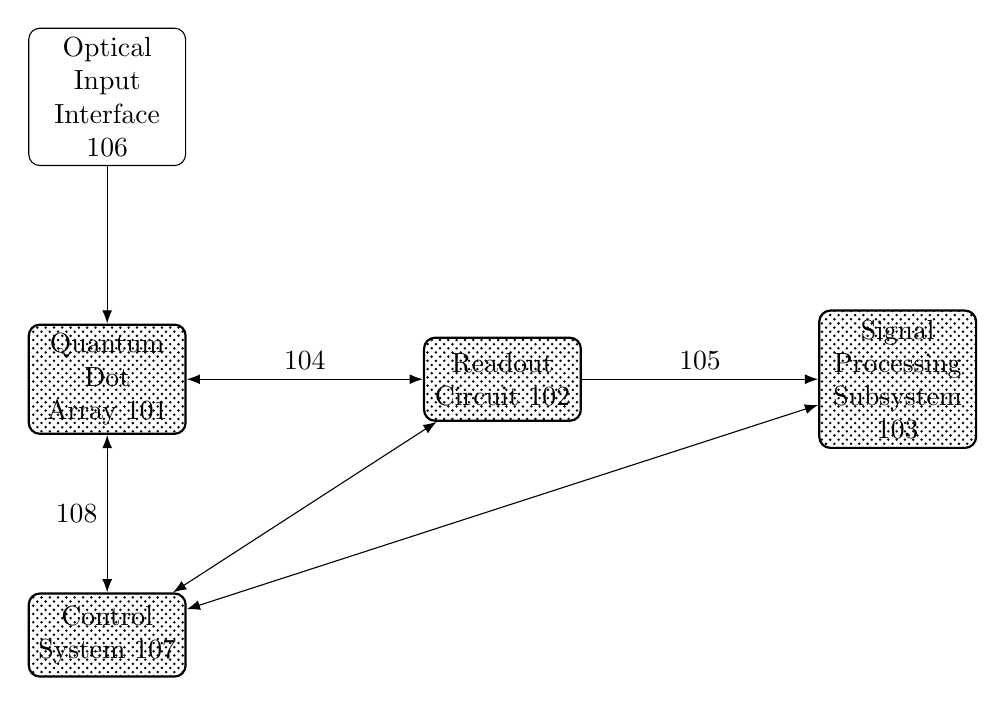
\begin{tikzpicture}[
    node distance=2cm and 3cm,
    block/.style={rectangle, draw, fill=white, text width=5em, text centered, rounded corners, minimum height=3em},
    mainblock/.style={rectangle, draw, fill=white, pattern=crosshatch dots, text width=5em, text centered, rounded corners, minimum height=3em, thick},
    line/.style={draw, -Latex},
    bidirectional/.style={draw, Latex-Latex}
    ]
    
    % Define nodes
    \node[block] (A) {Optical Input Interface 106};
    \node[mainblock, below=of A] (B) {Quantum Dot Array 101};
    \node[mainblock, right=of B] (C) {Readout Circuit 102};
    \node[mainblock, right=of C] (D) {Signal Processing Subsystem 103};
    \node[mainblock, below=of B] (E) {Control System 107};
    
    % Define connections
    \draw[line] (A) -- (B);
    \draw[bidirectional] (B) -- (C) node[midway, above] {104};
    \draw[line] (C) -- (D) node[midway, above] {105};
    \draw[bidirectional] (E) -- (B) node[midway, left] {108};
    \draw[bidirectional] (E) -- (C);
    \draw[bidirectional] (E) -- (D);
    
\end{tikzpicture}
\caption*{FIG. 1}
\end{figure}


\begin{figure}[h]
\centering
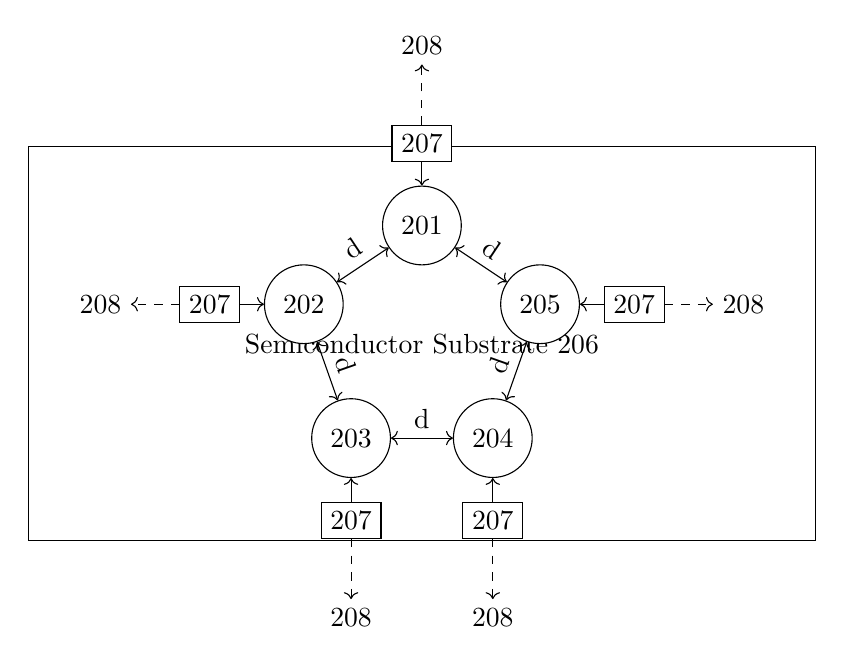
\begin{tikzpicture}[
    quantum dot/.style={circle, draw, fill=white, minimum size=1cm},
    electrode/.style={rectangle, draw, fill=white, minimum width=0.5cm, minimum height=0.2cm},
    substrate/.style={rectangle, draw, fill=white, minimum width=10cm, minimum height=5cm}
    ]
    
    % Draw substrate
    \node[substrate] (sub) at (0,0) {Semiconductor Substrate 206};
    
    % Draw quantum dots in pentagon arrangement
    \node[quantum dot] (qd1) at (0,1.5) {201};
    \node[quantum dot] (qd2) at (-1.5,0.5) {202};
    \node[quantum dot] (qd3) at (-0.9,-1.2) {203};
    \node[quantum dot] (qd4) at (0.9,-1.2) {204};
    \node[quantum dot] (qd5) at (1.5,0.5) {205};
    
    % Draw gate electrodes
    \node[electrode, above=0.3cm of qd1] (e1) {207};
    \node[electrode, left=0.3cm of qd2] (e2) {207};
    \node[electrode, below=0.3cm of qd3] (e3) {207};
    \node[electrode, below=0.3cm of qd4] (e4) {207};
    \node[electrode, right=0.3cm of qd5] (e5) {207};
    
    % Draw connection lines to electrodes
    \draw[->] (e1) -- (qd1);
    \draw[->] (e2) -- (qd2);
    \draw[->] (e3) -- (qd3);
    \draw[->] (e4) -- (qd4);
    \draw[->] (e5) -- (qd5);
    
    % Draw control lines
    \draw[->, dashed] (e1) -- ++(0,1) node[above] {208};
    \draw[->, dashed] (e2) -- ++(-1,0) node[left] {208};
    \draw[->, dashed] (e3) -- ++(0,-1) node[below] {208};
    \draw[->, dashed] (e4) -- ++(0,-1) node[below] {208};
    \draw[->, dashed] (e5) -- ++(1,0) node[right] {208};
    
    % Show optimal distances
    \draw[<->] (qd1) -- (qd2) node[midway, above, sloped] {d};
    \draw[<->] (qd2) -- (qd3) node[midway, above, sloped] {d};
    \draw[<->] (qd3) -- (qd4) node[midway, above] {d};
    \draw[<->] (qd4) -- (qd5) node[midway, above, sloped] {d};
    \draw[<->] (qd5) -- (qd1) node[midway, above, sloped] {d};
    
\end{tikzpicture}
\caption*{FIG. 2}
\end{figure}

\begin{figure}[h]
\centering
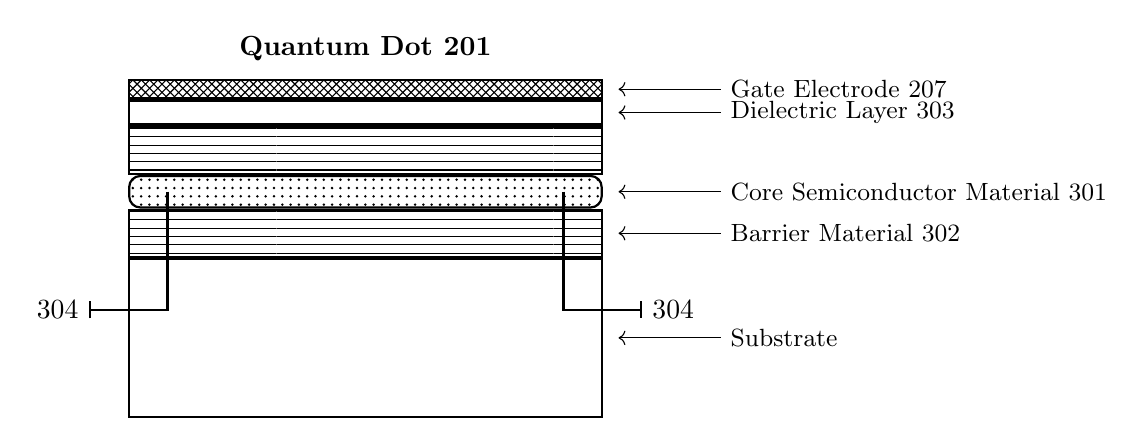
\begin{tikzpicture}[
    layer/.style={rectangle, draw, minimum width=6cm, thick},
    label/.style={font=\small}
    ]
    
    % Draw layers
    \node[layer, minimum height=2cm, fill=white] (substrate) at (0,0) {};
    \node[layer, minimum height=0.6cm, fill=white, pattern=horizontal lines, above=0cm of substrate] (barrier) {};
    \node[layer, minimum height=0.4cm, fill=white, pattern=dots, rounded corners, above=0cm of barrier] (core) {};
    \node[layer, minimum height=0.6cm, fill=white, pattern=horizontal lines, above=0cm of core] (barrier2) {};
    \node[layer, minimum height=0.3cm, fill=white, above=0cm of barrier2] (dielectric) {};
    \node[layer, minimum height=0.2cm, fill=white, pattern=crosshatch, above=0cm of dielectric] (gate) {};
    
    % Draw connecting leads
    \draw[thick, -|] ($(core.west) + (0.5,0)$) -- ++(0,-1.5) -- ++(-1,0) node[left] {304};
    \draw[thick, -|] ($(core.east) - (0.5,0)$) -- ++(0,-1.5) -- ++(1,0) node[right] {304};
    
    % Add labels with right alignment
    \node[label, right=1.5cm of gate] (gate_label) {Gate Electrode 207};
    \node[label, right=1.5cm of dielectric] (dielectric_label) {Dielectric Layer 303};
    \node[label, right=1.5cm of core] (core_label) {Core Semiconductor Material 301};
    \node[label, right=1.5cm of barrier] (barrier_label) {Barrier Material 302};
    \node[label, right=1.5cm of substrate] (substrate_label) {Substrate};
    
    % Add arrows connecting labels to layers
    \draw[<-] ($(gate.east) + (0.2,0)$) -- ++(1.3,0);
    \draw[<-] ($(dielectric.east) + (0.2,0)$) -- ++(1.3,0);
    \draw[<-] ($(core.east) + (0.2,0)$) -- ++(1.3,0);
    \draw[<-] ($(barrier.east) + (0.2,0)$) -- ++(1.3,0);
    \draw[<-] ($(substrate.east) + (0.2,0)$) -- ++(1.3,0);
    
    % Add quantum dot label
    \node[above=0.1cm of gate, font=\bfseries] {Quantum Dot 201};
    
\end{tikzpicture}
\caption*{FIG. 3}
\end{figure}

\begin{figure}[h]
\centering
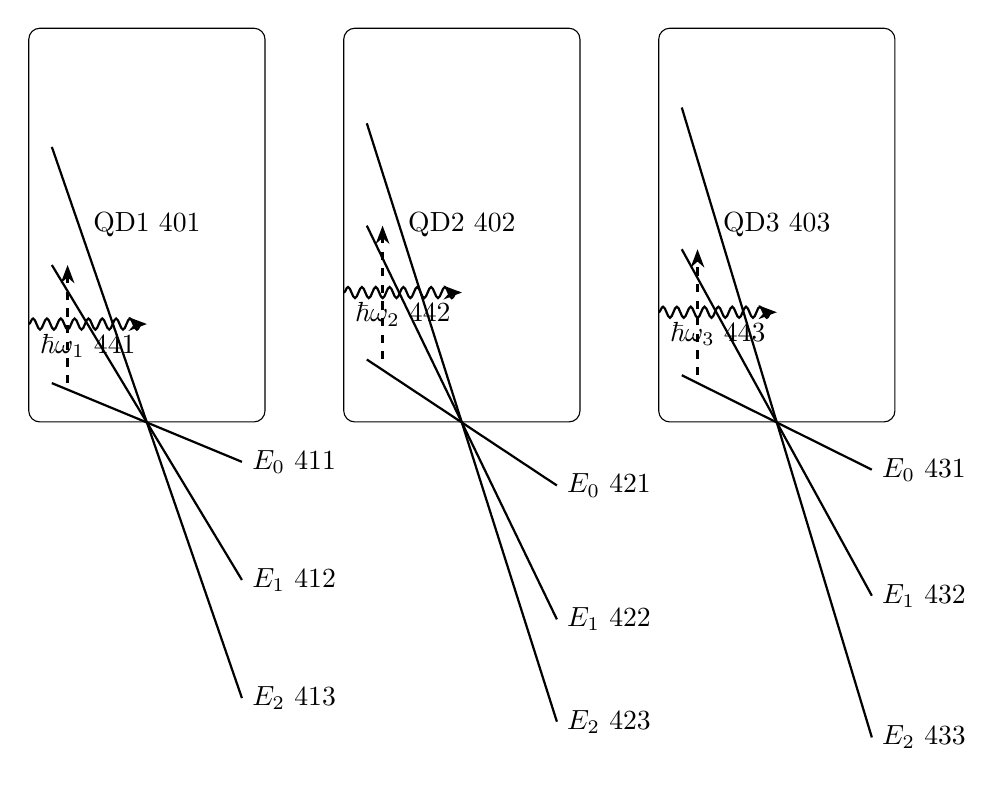
\begin{tikzpicture}[
    energy level/.style={thick, draw=black},
    quantum dot/.style={rectangle, draw, rounded corners, minimum width=3cm, minimum height=5cm, fill=white},
    transition/.style={->, >=Stealth, thick, dashed},
    photon/.style={->, >=Stealth, thick, decorate, decoration={snake, amplitude=2pt, segment length=5pt}}
    ]
    
    % Define quantum dots
    \node[quantum dot] (qd1) at (0,0) {QD1 401};
    \node[quantum dot] (qd2) at (4,0) {QD2 402};
    \node[quantum dot] (qd3) at (8,0) {QD3 403};
    
    % Define energy levels for QD1
    \draw[energy level] ($(qd1.south west) + (0.3,0.5)$) -- ($(qd1.south east) - (0.3,0.5)$) node[right] {$E_0$ 411};
    \draw[energy level] ($(qd1.south west) + (0.3,2)$) -- ($(qd1.south east) - (0.3,2)$) node[right] {$E_1$ 412};
    \draw[energy level] ($(qd1.south west) + (0.3,3.5)$) -- ($(qd1.south east) - (0.3,3.5)$) node[right] {$E_2$ 413};
    
    % Define energy levels for QD2
    \draw[energy level] ($(qd2.south west) + (0.3,0.8)$) -- ($(qd2.south east) - (0.3,0.8)$) node[right] {$E_0$ 421};
    \draw[energy level] ($(qd2.south west) + (0.3,2.5)$) -- ($(qd2.south east) - (0.3,2.5)$) node[right] {$E_1$ 422};
    \draw[energy level] ($(qd2.south west) + (0.3,3.8)$) -- ($(qd2.south east) - (0.3,3.8)$) node[right] {$E_2$ 423};
    
    % Define energy levels for QD3
    \draw[energy level] ($(qd3.south west) + (0.3,0.6)$) -- ($(qd3.south east) - (0.3,0.6)$) node[right] {$E_0$ 431};
    \draw[energy level] ($(qd3.south west) + (0.3,2.2)$) -- ($(qd3.south east) - (0.3,2.2)$) node[right] {$E_1$ 432};
    \draw[energy level] ($(qd3.south west) + (0.3,4.0)$) -- ($(qd3.south east) - (0.3,4.0)$) node[right] {$E_2$ 433};
    
    % Draw transitions with photons
    \draw[transition] ($(qd1.south west) + (0.5,0.5)$) -- ($(qd1.south west) + (0.5,2)$);
    \draw[photon] ($(qd1.south) + (-1.5,1.25)$) -- ($(qd1.south) + (0,1.25)$) node[midway, below] {$\hbar\omega_1$ 441};
    
    \draw[transition] ($(qd2.south west) + (0.5,0.8)$) -- ($(qd2.south west) + (0.5,2.5)$);
    \draw[photon] ($(qd2.south) + (-1.5,1.65)$) -- ($(qd2.south) + (0,1.65)$) node[midway, below] {$\hbar\omega_2$ 442};
    
    \draw[transition] ($(qd3.south west) + (0.5,0.6)$) -- ($(qd3.south west) + (0.5,2.2)$);
    \draw[photon] ($(qd3.south) + (-1.5,1.4)$) -- ($(qd3.south) + (0,1.4)$) node[midway, below] {$\hbar\omega_3$ 443};
    
\end{tikzpicture}
\caption*{FIG. 4}
\end{figure}

\begin{figure}[h]
\centering
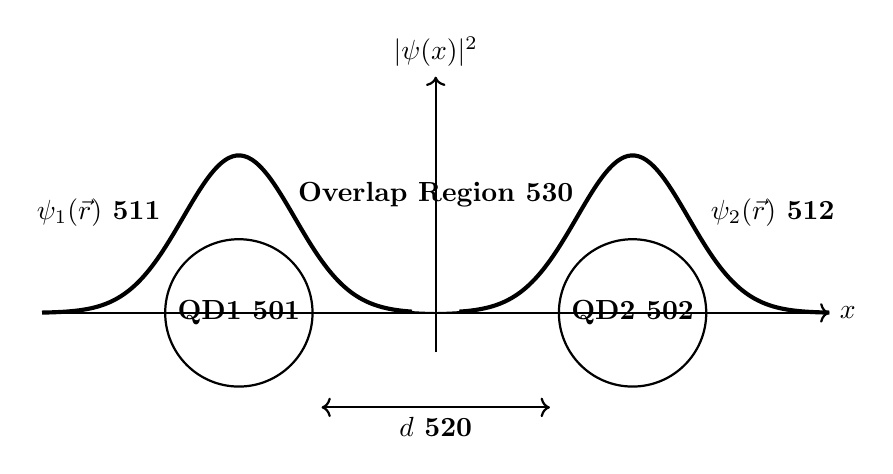
\begin{tikzpicture}[
    quantum dot/.style={circle, draw, thick, minimum size=1.5cm, font=\bfseries},
    wavefunction/.style={thick},
    ]
    
    % Draw coordinate axis
    \draw[->, thick] (-5,0) -- (5,0) node[right, font=\bfseries] {$x$};
    \draw[->, thick] (0,-0.5) -- (0,3) node[above, font=\bfseries] {$|\psi(x)|^2$};
    
    % Draw quantum dots
    \node[quantum dot] (qd1) at (-2.5,0) {QD1 501};
    \node[quantum dot] (qd2) at (2.5,0) {QD2 502};
    
    % Draw distance between dots
    \draw[<->, thick] ($(qd1.east) + (0.1,-1.2)$) -- ($(qd2.west) + (-0.1,-1.2)$) node[midway, below, font=\bfseries] {$d$ 520};
    
    % Draw wavefunctions
    \draw[wavefunction, domain=-5:-0.3, samples=100, smooth, line width=1.5pt] 
        plot (\x, {2*exp(-(\x+2.5)*(\x+2.5)/1)});
    \node[font=\bfseries, above left=0.3cm and 0.2cm of qd1] {$\psi_1(\vec{r})$ 511};
        
    \draw[wavefunction, domain=0.3:5, samples=100, smooth, line width=1.5pt] 
        plot (\x, {2*exp(-(\x-2.5)*(\x-2.5)/1)});
    \node[font=\bfseries, above right=0.3cm and 0.2cm of qd2] {$\psi_2(\vec{r})$ 512};
    
    % Draw overlap region with hatching instead of color
    \draw[pattern=north east lines, pattern color=black] 
        plot[domain=-0.3:0.3, samples=50, smooth] 
        (\x, {2*exp(-(\x+2.5)*(\x+2.5)/1)}) -- 
        plot[domain=0.3:-0.3, samples=50, smooth] 
        (\x, {2*exp(-(\x-2.5)*(\x-2.5)/1)}) -- cycle;
    
    % Label overlap region
    \node[font=\bfseries, align=center, text width=4cm] at (0,1.5) {Overlap Region 530};
    
\end{tikzpicture}
\caption*{FIG. 5}
\end{figure}

\begin{figure}[h]
\centering
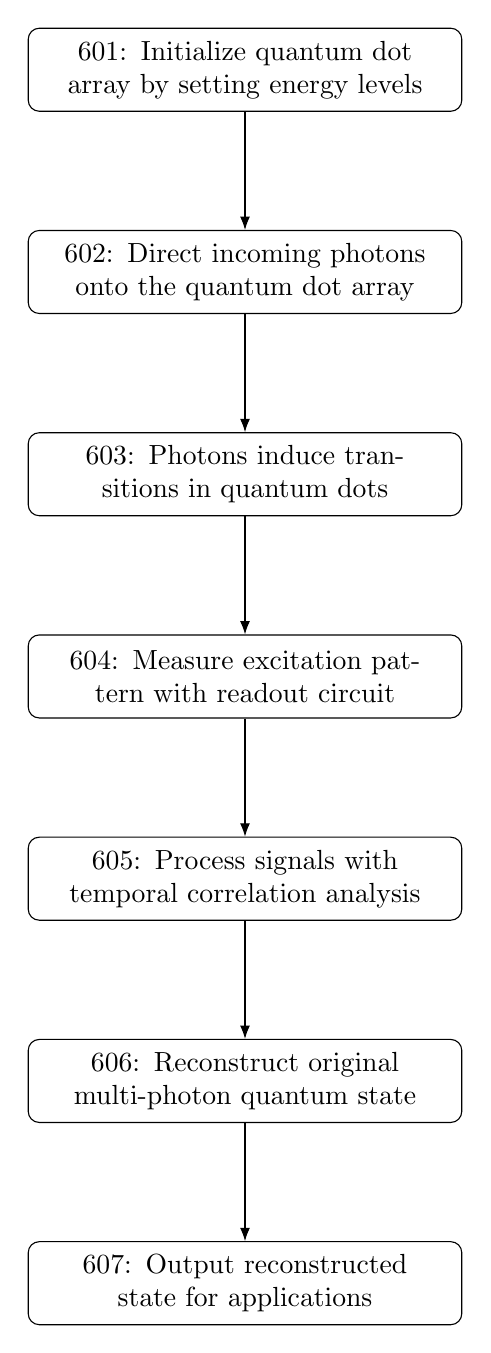
\begin{tikzpicture}[
node distance=1.5cm,
block/.style={rectangle, draw, fill=white, text width=15em, text centered, rounded corners, minimum height=3em},
line/.style={draw, -Latex}
]

% Define nodes
\node[block] (A) {601: Initialize quantum dot array by setting energy levels};
\node[block, below=of A] (B) {602: Direct incoming photons onto the quantum dot array};
\node[block, below=of B] (C) {603: Photons induce transitions in quantum dots};
\node[block, below=of C] (D) {604: Measure excitation pattern with readout circuit};
\node[block, below=of D] (E) {605: Process signals with temporal correlation analysis};
\node[block, below=of E] (F) {606: Reconstruct original multi-photon quantum state};
\node[block, below=of F] (G) {607: Output reconstructed state for applications};

% Define connections
\draw[line] (A) -- (B);
\draw[line] (B) -- (C);
\draw[line] (C) -- (D);
\draw[line] (D) -- (E);
\draw[line] (E) -- (F);
\draw[line] (F) -- (G);

\end{tikzpicture}
\caption*{FIG. 6}
\end{figure}

\begin{figure}[h]
\centering
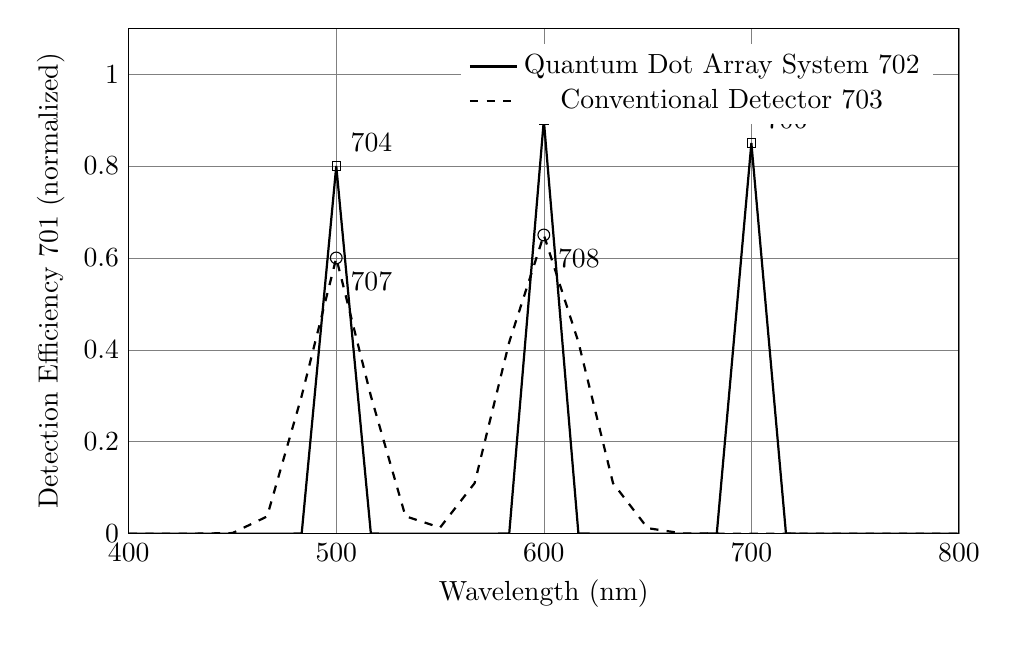
\begin{tikzpicture}
\begin{axis}[
    width=\linewidth,
    height=8cm,
    xlabel={Wavelength (nm)},
    ylabel={Detection Efficiency 701 (normalized)},
    xmin=400, xmax=800,
    ymin=0, ymax=1.1,
    xtick={400,500,600,700,800},
    ytick={0,0.2,0.4,0.6,0.8,1.0},
    legend pos=north east,
    legend style={draw=none},
    grid=both,
    grid style={line width=.1pt, draw=black!10},
    major grid style={line width=.2pt,draw=black!50},
]
% Quantum Dot Array Response - solid line
\addplot[domain=400:800, thick, black] {0.8*exp(-((x-500)/5)^2) + 0.9*exp(-((x-600)/5)^2) + 0.85*exp(-((x-700)/5)^2)};
\addlegendentry{Quantum Dot Array System 702}

% Conventional Detector Response - dashed line
\addplot[domain=400:800, thick, black, dashed] {0.6*exp(-((x-500)/20)^2) + 0.65*exp(-((x-600)/25)^2)};
\addlegendentry{Conventional Detector 703}

% Add peak labels for quantum dot array - using square markers
\node[rectangle, draw, inner sep=1.5pt, label={above right:704}] at (axis cs:500,0.8) {};
\node[rectangle, draw, inner sep=1.5pt, label={above right:705}] at (axis cs:600,0.9) {};
\node[rectangle, draw, inner sep=1.5pt, label={above right:706}] at (axis cs:700,0.85) {};

% Add peak labels for conventional detector - using circular markers
\node[circle, draw, inner sep=1.5pt, label={below right:707}] at (axis cs:500,0.6) {};
\node[circle, draw, inner sep=1.5pt, label={below right:708}] at (axis cs:600,0.65) {};

\end{axis}
\end{tikzpicture}
\caption*{FIG. 7}
\end{figure}

\begin{figure}[h]
\centering
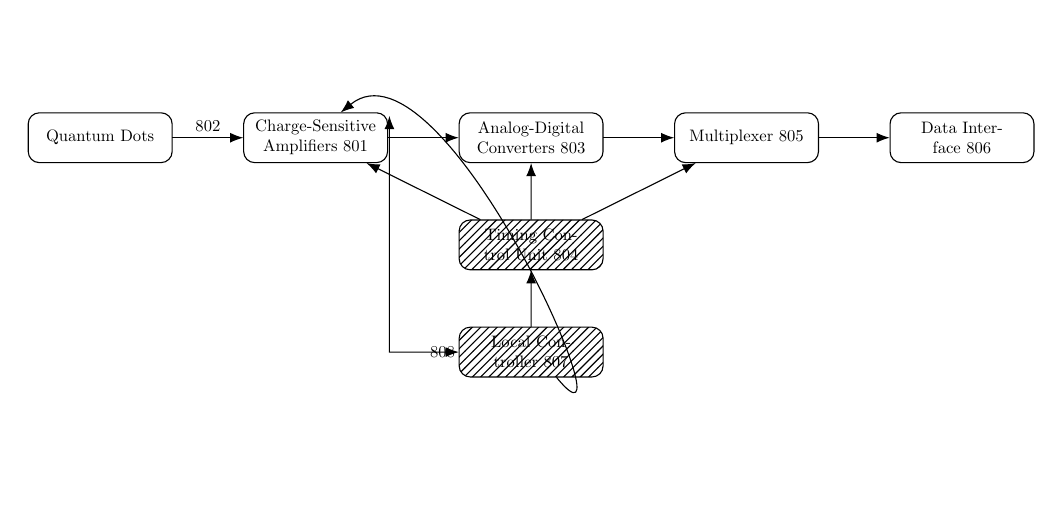
\begin{tikzpicture}[scale=0.6, transform shape,
node distance=1.2cm and 1.5cm,
block/.style={rectangle, draw, fill=white, text width=8em, text centered, rounded corners, minimum height=3em},
controlblock/.style={rectangle, draw, fill=white, pattern=north east lines, text width=8em, text centered, rounded corners, minimum height=3em},
line/.style={draw, -Latex},
bidirectional/.style={draw, Latex-Latex}
]

% Define main signal path
\node[block] (A) {Quantum Dots};
\node[block, right=of A] (B) {Charge-Sensitive Amplifiers 801};
\node[block, right=of B] (C) {Analog-Digital Converters 803};
\node[block, right=of C] (D) {Multiplexer 805};
\node[block, right=of D] (E) {Data Interface 806};

% Define control elements
\node[controlblock, below=of C] (F) {Timing Control Unit 804};
\node[controlblock, below=of F] (G) {Local Controller 807};

% Define main signal flow
\draw[line] (A) -- (B) node[midway, above] {802};
\draw[line] (B) -- (C);
\draw[line] (C) -- (D);
\draw[line] (D) -- (E);

% Define control flows
\draw[line] (F) -- (B);
\draw[line] (F) -- (C);
\draw[line] (F) -- (D);
\draw[line] (G) -- (F);
\draw[line, bend right] (G) to[out=180,in=270] (B);
\draw[bidirectional] (G) -- node[right] {808} ++(-3,0) -- ++(0,5);

\end{tikzpicture}
\caption*{FIG. 8}
\end{figure}

\begin{figure}[h]
\centering
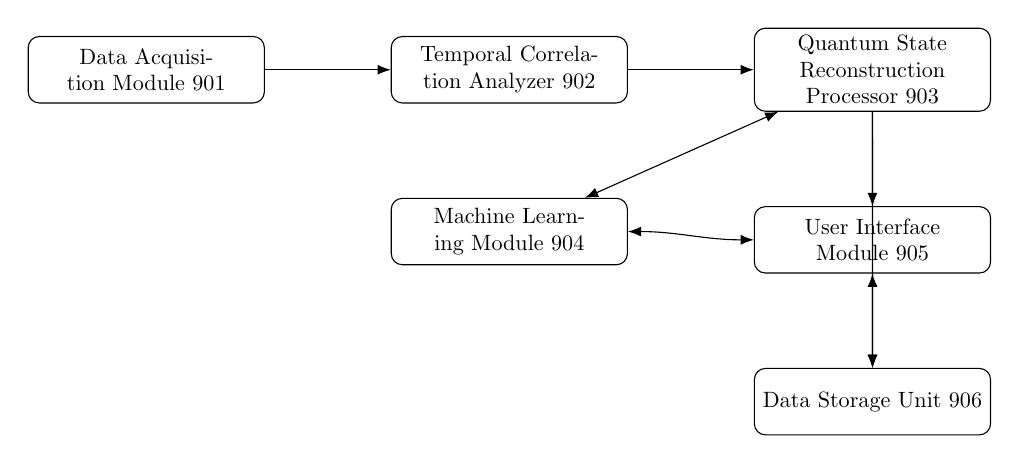
\begin{tikzpicture}[scale=0.8, transform shape,
node distance=1.5cm and 2cm,
block/.style={rectangle, draw, fill=white, text width=10em, text centered, rounded corners, minimum height=3em},
line/.style={draw, -Latex},
bidirectional/.style={draw, Latex-Latex}
]

% Define main processing pipeline
\node[block] (A) {Data Acquisition Module 901};
\node[block, right=of A] (B) {Temporal Correlation Analyzer 902};
\node[block, right=of B] (C) {Quantum State Reconstruction Processor 903};

% Define auxiliary modules
\node[block, below=of B] (D) {Machine Learning Module 904};
\node[block, below=of C] (E) {User Interface Module 905};
\node[block, below=of E] (F) {Data Storage Unit 906};

% Define connections
\draw[line] (A) -- (B);
\draw[line] (B) -- (C);
\draw[bidirectional] (D) -- (C);
\draw[line] (C) -- (E);
\draw[line] (C) -- (F);
\draw[bidirectional] (D) to[out=0,in=180] (E);
\draw[bidirectional] (E) -- (F);

\end{tikzpicture}
\caption*{FIG. 9}
\end{figure}

\begin{figure}[h]
\centering
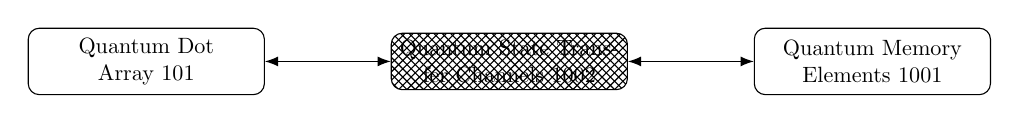
\begin{tikzpicture}[scale=0.8, transform shape,
    node distance=1.5cm and 2cm,
    block/.style={rectangle, draw, fill=white, text width=10em, text centered, rounded corners, minimum height=3em},
    channel/.style={rectangle, draw, fill=white, pattern=crosshatch, text width=10em, text centered, rounded corners, minimum height=2.5em},
    line/.style={draw, -Latex},
    bidirectional/.style={draw, Latex-Latex}
    ]
    
    % Define nodes
    \node[block] (A) {Quantum Dot Array 101};
    \node[channel, right=of A] (B) {Quantum State Transfer Channels 1002};
    \node[block, right=of B] (C) {Quantum Memory Elements 1001};
    
    % Define connections
    \draw[bidirectional] (A) -- (B);
    \draw[bidirectional] (B) -- (C);
    
\end{tikzpicture}
\caption*{FIG. 10}
\end{figure}

\end{document}